\section{The MS-GAT Model}
\label{sec:the_ms-gat_model}

Following the problem statement and the framework of modeling traffic signal couplings in Section \ref{sec:problem_statement}, MS-GAT instantiates a concrete mapping network $f_G$ for traffic prediction, as shown in Fig.~\ref{fig:framework}. MS-GAT captures three-dimensional relations and their interactions on nodes of traffic network: i) the spatial and temporal relations among nodes; ii) the channel relations between traffic signal channels which influence the evolution of the whole traffic conditions on a road network; and iii) the distinct importance of each kind of relations to future traffic conditions of an individual node. Below, we introduce the network architecture, multi-dimensional self-attention, and multi-correlation embedding to model the multivariate and multi-relational traffic network, repsectively. 

\subsection{The Network Architecture}
\label{ssec:the_network_architecture}

\subsubsection{Overview}
The MS-GAT model is composed of $M$ same traffic prediction components (\textit{TPC} for short) and adopts a multi-component structure based on the time-gated fusion. To achieve more accurate short-term prediction with a less parameter scale for efficient real-time prediction results, each \textit{TPC} component is designed to share an identical network structure. The shared network structure follows the light-head structural style, which has proved very efficient in such computer vision tasks as target detection \cite{li2017light}, rather than leveraging a heavy encoder-decoder framework.

As shown in the left part of Fig.~\ref{fig:framework}, each \textit{TPC} consists of multiple stacked \underline{m}ulti-relational \underline{e}mbedding \underline{a}breast \underline{m}odules (MEAMs for short), and a light-head block associated with ultimate prediction. In a \textit{TPC}, the MEAM stacking replicas are responsible for extracting the complex dynamic features related to various dependencies among traffic conditions from the input data to the current \textit{TPC}. Subsequently, a light-head block is attached to its previous MEAMs to straightforwardly accomplish the mapping (regression) of the learned deep features to prediction results. Here, the light-head block is a sequential composition of two canonical operations, namely \textit{Layer Normalization} and \textit{Fully Connection}, for avoiding the heavy decoding overhead under the premise of ensuring the accuracy of short-term prediction. Formally, the input and output of the $i^{th}$ ($1 \leq i \leq \mathit{M}$) \textit{TPC} are  denoted as samples $x_i \in \mathbb{R}^{C \times N \times P_i}$ and output $\hat{y_i} \in \mathbb{R}^{C \times N \times Q_i}$ respectively, where $C$ denotes the number of channels at a single traffic node, $N$ denotes the number of traffic nodes, $P_i$ and $Q_i$ refer to the time steps respectively associated with the input samples and prediction results of the $i^{th}$ \textit{TPC}. Here, $i$ refers to the identification number of a \textit{TPC} in the proposed model adopting multi-component structure.  

\subsubsection{Multi-component structure based on time-gated fusion}

According to the formal statement in Equation~\ref{eqn:target_function}, the traffic prediction issue is naturally regarded as a seq2seq learning task. However, for a seq2seq model by supervised learning, we find: i) feeding it with longer historical sequential data at one time may lead to the rise of model overhead but does not necessarily improve the accuracy of forecasted sequence; ii) different historical segments with same sequence length but distinct offsets to the common ‘\textit{now}’ moment show separate importances to the identical future sequence. These show the sensitivity of the length and starting and ending points of a training sequence on the accuracy and efficiency of forecasting the output by a seq2seq model. To address these issues, MS-GAT adopts the ensemble learning and multi-component architectural style to its design and training.

In MS-GAT, the $i^{th}$ \textit{TPC} acts as a separate sub-model that corresponds to a learnable mapping function $f_i$. Importantly, despite all \textit{TPCs} take the same length of time-series graph signals as their input sequences, they deal with respective time slices that have different offsets relative to the same present moment. In detail, as shown in Fig.~\ref{fig:sampling}, we pick up \textit{M} shorter time sequences from the past \textit{P}-step graph signals according to their importance for the next \textit{Q}-step traffic conditions, each of which behaves as the input samples of different \textit{TPCs}. Formally, for the input sequence of the $i^{th}$ \textit{TPC}, $x_i=(x_i^1, x_i^2, \cdots ,x_i^r) \in \mathbb{R}^{C \times N \times r}$, where $r$ refers to the length of time steps of input samples (apparently, here $r$ equals  $P_i$), and each $x_i^\eta (1 \leq \eta \leq r)$ corresponds to a separate graph signal on the traffic network depicting the traffic condition at a specified moment. Moreover, the starting time point of $x_i$ is denoted as $t(x_i^1)$, and $|t(x_i^1) - t_{now}|$ corresponds to the offset of $x_i$ relative to the specified present moment denoted as $t_{now}$. Accordingly, the input samples of MS-GAT is as follows: $x = [x_1, \dots , x_M] \in \mathbb{R}^{M \times C \times N \times r}$.

\begin{figure}[!ht]
    \centering
    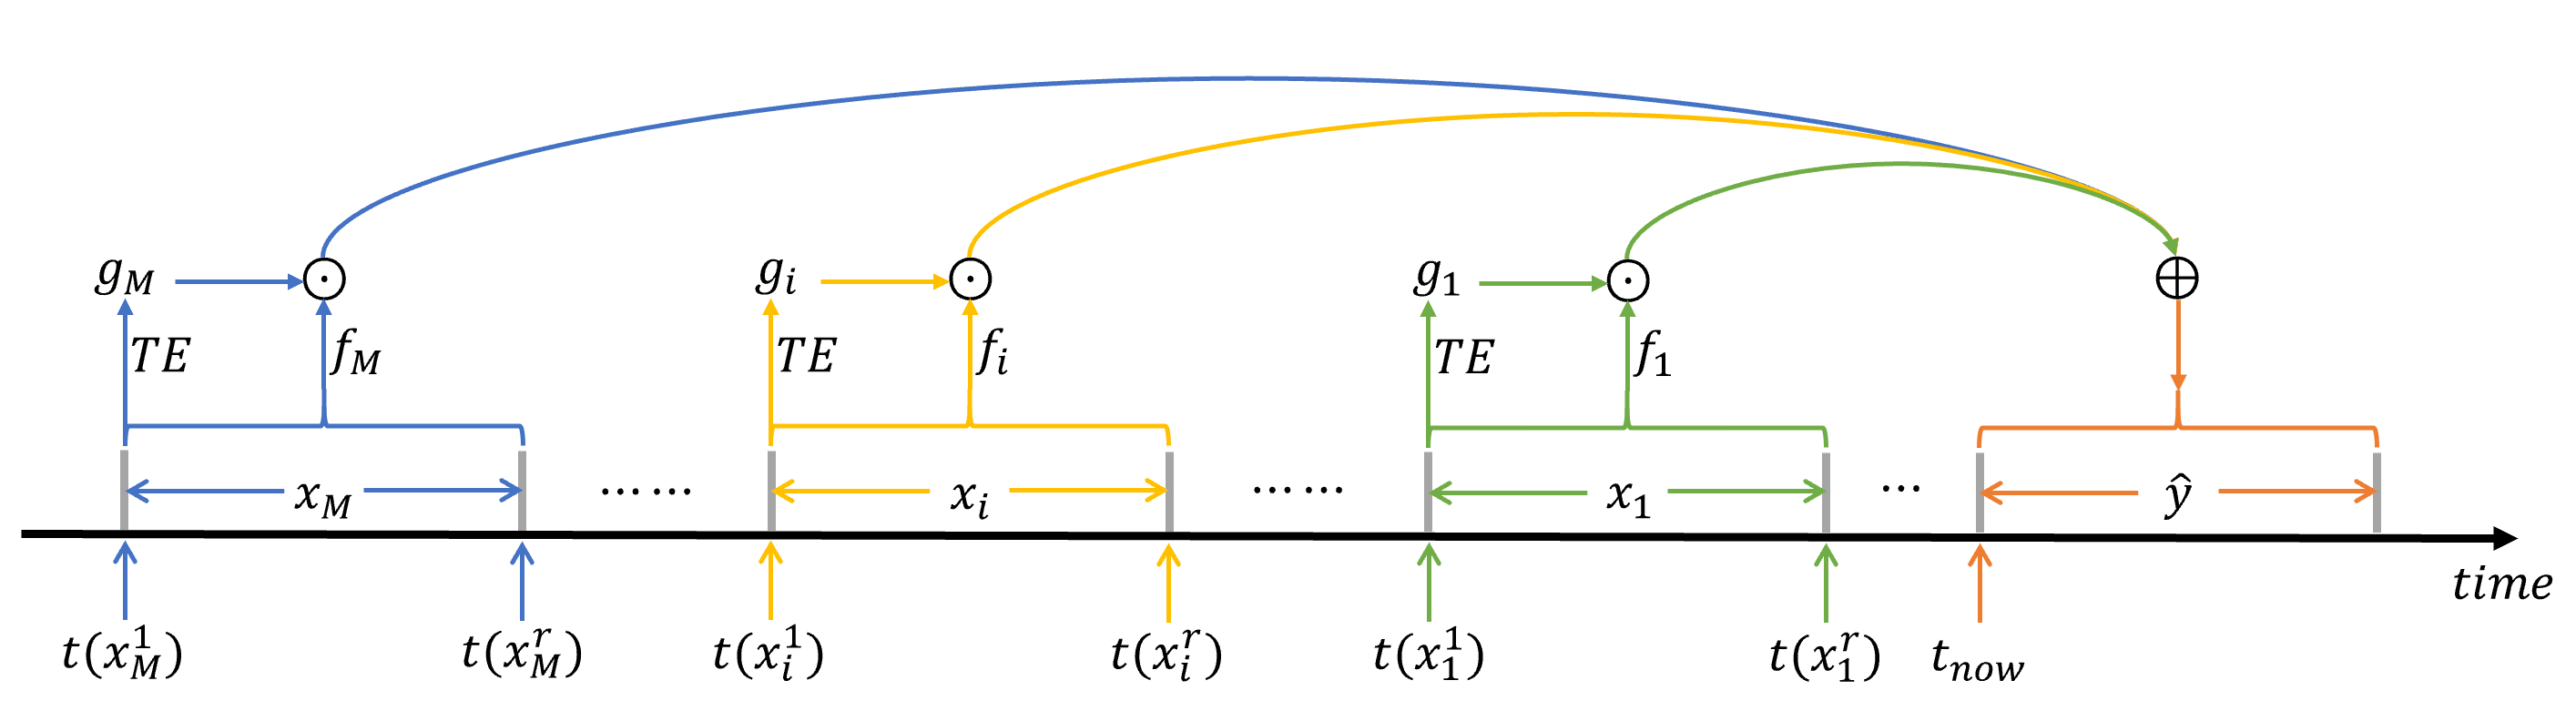
\includegraphics[width=0.48\textwidth]{pictures/Sampling.png}
    \caption{Illustration of the sampling window that slides over the entire time-series graph signals}
    \label{fig:sampling}
\end{figure}

Meanwhile, when the specified present moment $t_{now}$ moving over the whole observed historical graph signals along the time axis, the past $P$ time steps together with the next  $Q$ time steps form a sliding window to generate training samples for our model. As a result, a rich number of distinct training samples can be flexibly yielded from a small historical time-series data in this manner, which evidently improves the capability of the regression model.

\textit{Time embedding for the gated fusion}. 
It is observed that the traffic conditions at the past distinct time slices have different correlation strengths with that of the same future time slice. Accordingly, we propose to incorporate the time information of each input sequence $x_i$ into its corresponding mapping function $f_i(x_i)$ by adding a timing embedding module (called \textit{TE}) in each \textit{TPC} (shown in Fig.~\ref{fig:framework}), and further leverage a gated fusion mechanism to adaptively merge all sub-models (\textit{TPCs}) to obtain an ultimate prediction model based on the multi-component structure, i.e., MS-GAT. To be specific, by using one-hot coding, we encode the day-of-week and time-of-day of the starting time point $t(x_i^1)$ of each input sequence $x_i$ into the vectors $D_i \in R^7$ and $H_i \in R^{24}$, respectively. After that, by applying a vector embedding approach (e.g., word2vec \cite{church2017word2vec}), the two vectors are transformed to two other vectors with the same dimension, respectively. They are then added together forming the time embedding of the input sequence $x_i$. Formally, the time embedding related to the input sequence $x_i$ corresponds to a tensor denoted as $g_i$, which will be fused as a gate with the associated mapping function $f_i(x_i)$. Thus, the final prediction result after the fusion is:

\begin{equation}
    \label{eqn:gate_fusion}
    \hat{y} = \sum\limits_{i=1}^{M}g_i \odot f_i(x_i),
\end{equation}

where

\begin{equation}
    \label{eqn:time_embedding}
    g_i = TE(D_i, H_i),
\end{equation}

$\odot$ represents the element-wise product, the function $TE(\cdot)$ denotes the specific implementation of the above embedding process related with the timing embedding module called \textit{TE}, both $f_i(\cdot)$ and function $TE(\cdot)$ contain learnable parameters, $g_i \in \mathbb{R}^{C \times N \times Q}$, and $f_i(x_i) \in \mathbb{R}^{C \times N \times Q}$.

\subsection{Multi-dimensional self-attention scheme}
\label{ssec:multi-dimensional_self-attention_scheme}

We first briefly review an ordinary self-attention scheme, called scaled dot-product attention \cite{vaswani2017attention}, which adopts ordinary dot-product between vectors as the core operation of whole self-attention process to obtain the correlation strength between input vectors, i.e., \textit{attention score}. 


\begin{figure}[!ht]
    \centering
    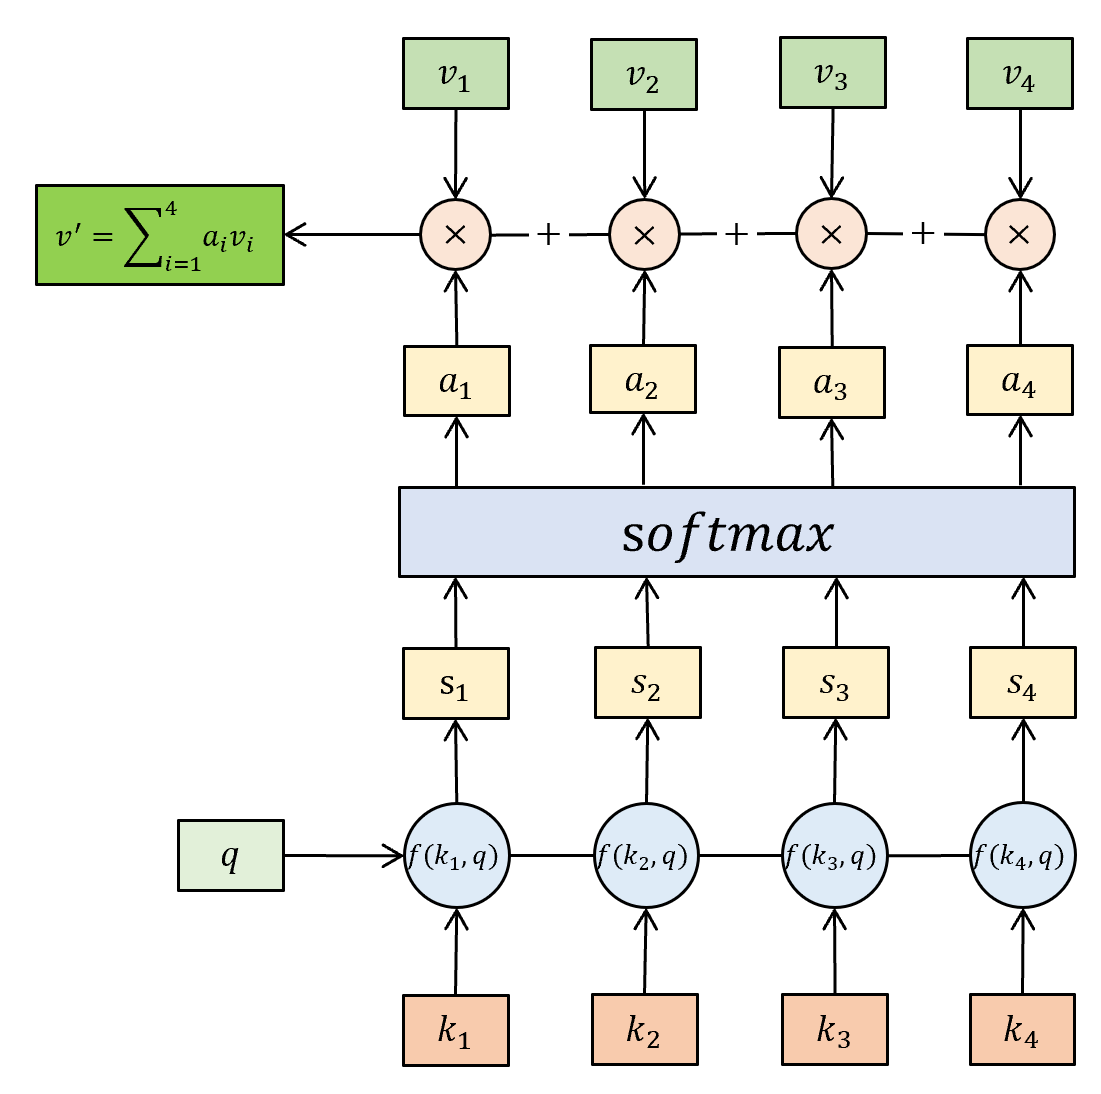
\includegraphics[width=0.32\textwidth]{pictures/Attention.png}
    \caption{The calculation process of self-attention in an exemplar sentence - \textit{this is a cat}. Here, $q$ refers to the \textit{query} vector associated with the word ‘this’, ‘is’, ‘a’ or ‘cat’; $(k_1, v_1)$, $(k_2, v_2)$, $(k_3, v_3)$ and $(k_4, v_4)$ represent the \textit{key-value} pairs of the four separate words respectively; $f$ denotes a type of attention function that adopts dot-product operation between two vectors (i.e., the above \textit{key} and \textit{query}), and $s_1$, $s_2$, $s_3$ and $s_4$ are its resulting attention scores respectively; the $softmax$ function is used to normalize these attention score to $a_1$, $a_2$, $a_3$ and $a_4$ respectively, which are all in the range of $[0, 1]$; $v'$ is the result of current word after performing self-attention by its associated $q$, which contains the contexts of this sentence except for the information of current word itself.}
    \label{fig:attention}
\end{figure}


Taking a linguistic sentence, e.g., \textit{this is a cat}, as an example. Clearly, it is a sequence of words, and can be viewed as a sequential data just over temporal dimension. Importantly, this sentence also conceals the contextual dependencies in temporal dimension between these four separate words. To find out such hidden dependency relations from this sentence, valuable for the tasks of NLP (e.g., language translation), the ordinary attention scheme can be alone applied in a specified information dimension, i.e., temporal dimension of this sequential data. Concretely, each word of the sentence is initially embedded to a vector by a vectorization method (e.g., classic word2vec \cite{church2017word2vec}), and further three same vectors (called query, key and value respectively) derived from the previous vector by linear transform are inputted simultaneously into the self-attention module. After each query of this sentence (i.e., corresponding to each word respectively) accomplishes self-attention operation with all of four key-value pairs, an output sequential data is obtained, which exposes those potential significant contexts into its each sequential element. Figure~\ref{fig:attention} shows the calculation process of this self-attention scheme in the exemplar sentence. Formally, given a query $q$, all keys (packed into matrices $K$) and values (packed into matrices $V$), the output value $value$ is weighted average over the input values as below.

\begin{equation}
    \label{eqn:attention_1}
    value = softmax(\frac{q K^\top}{\sqrt{d_k}}) V
\end{equation}

where $d_k$ is the dimension of $K$, the weights are the outputs of a \textit{softmax} function, and the inputs of the \textit{softmax} function are scaled dot products of the queries with all keys. Furthermore, when a sequence of queries is also combined in matrices form $Q$, the attention map, i.e., a resultant matrix including all attention scores, is calculated by Equation~\ref{eqn:attention_2}.

\begin{equation}
    \label{eqn:attention_2}
    Attention(Q,K,V) = softmax(\frac{Q K^\top}{\sqrt{d_k}}) V
\end{equation}

When only two aspects of information in the original input data, e.g., spatial-relevant and temporal-relevant information of normal spatio-temporal data, are attended to, the canonical attention scheme seems easy to carry out in a learning model. The existing traffic prediction models relying on attention mechanism (e.g., \cite{guo2019attention,zheng2020gman}) mostly act in accordance with this scheme. However, if there are more aspects of information to be focused on, the ordinary scheme is not convenient to be deployed. Specifically, when the self-attention is separately paid to each aspect of information, every associated dimension in the input data needs to alternatively apply the above scheme, which would result in such dilemmas as the large parameter scale and the code-level redundancy, thus affecting the model performance. Therefore, we seek a better attention implementation way to capture those correlations when more aspects of information need to be considered from their associated multi-dimensional data.

In MS-GAT, we develop a simple yet effective multi-dimensional self-attention scheme to enable the convenient generalization of existing ordinary self-attention scheme to a multi-dimensional information space. Notably, the proposed scheme is formulated as a reusable process, which is good at being universally and conveniently carried out in various information dimension of a multi-dimensional data, even with less computational cost for the resultant model. It works as follows.

\begin{figure}[!ht]
    \centering
    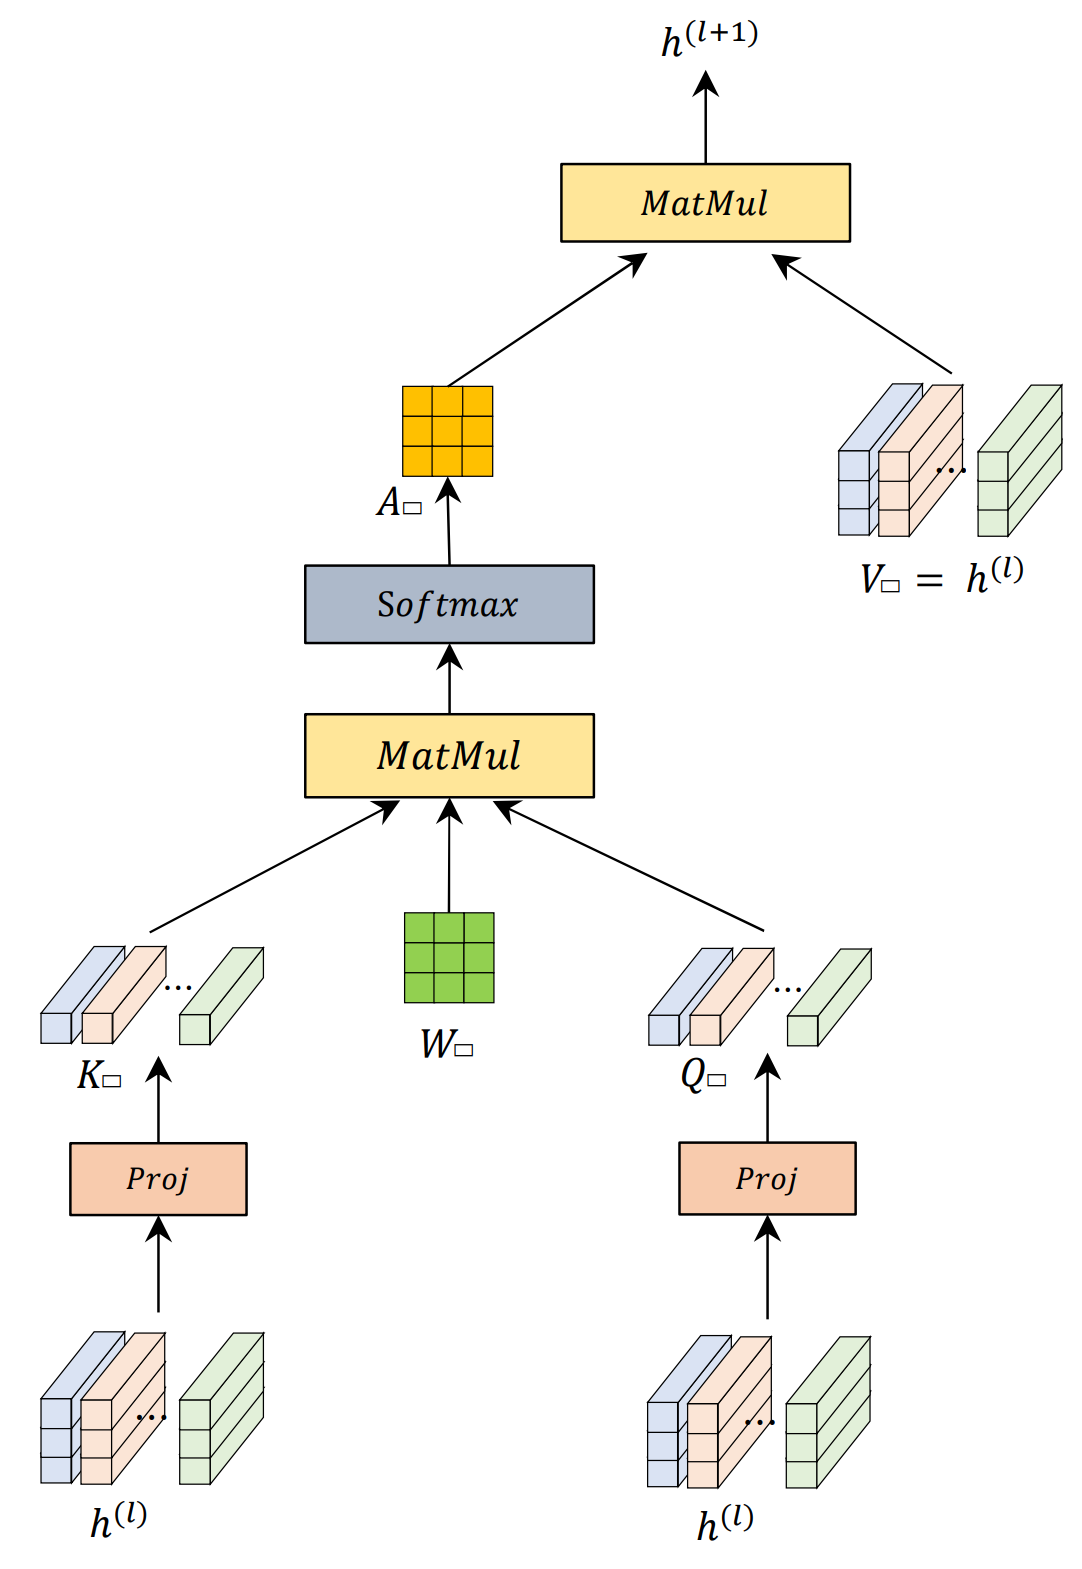
\includegraphics[width=0.4\textwidth]{pictures/Multidim_Attention.png}
    \caption{Illustration of the calculation process of our multi-dimensional self-attention scheme. Here, \textit{MatMul} refers to matrix multiplication; \textit{Proj} denotes the operation of linear transformation; $Q_{_\square}$, $K_{_\square}$ and $V_{_\square}$ are the query, key and value in the multi-dimensional self-attention respectively; $h^{(l)}$ and $h^{(l+1)}$ are the input and output of the $l^{th}$ layer multi-dimensional self-attention. }
    \label{fig:multidim_attention}
\end{figure}

Taking a three-dimensional space including the $x-$, $y-$ and $z-$axes as an example, which represent three different aspects of information associated with the original data, respectively. As a matter of fact, x-axis, y-axis and z-axis can correspond to the spatial, temporal and channel dimensions of spatio-temporal traffic signal data respectively. For the ease of description, the exemplar data space is denoted as a discrete set $\{h_{x,y,z}\}$, each element  $h_{x,y,z}$ is represented in a three-dimensional subscript form. Suppose that the potential correlation inside the information along the $x-$axis needs to be caught, the information separately along the other two dimensions (i.e., $y-$ and $z-$axes) will work together to achieve it. To be specific, our self-attention scheme sets query, key and value to the identical matrix denoted as $h_{x,:,:}$, where the subscript ‘$:$’ denotes all elements in the corresponding dimension, rather than the vector in the prior ordinary self-attention scheme. For instance, as for diverse spatio-temporal traffic signals throughout a road network, when only different kinds of traffic signals at a certain traffic node are considered, these traffic signal data (e.g., traffic flow, speed and occupancy at a location) within some time range form such a 2-D matrix called query, key or value, owing to their involved information of both temporal and channel dimensions. In addition, if it is a four-dimensional data space, three of them can be set in the tensor form, and so on for the higher-dimensional space. Afterwards, both query and key are transformed to their associated vectors respectively by employing an efficient linear transformation without parameters for tensor operation (e.g., the general API function \textit{torch.einsum()} can be used for the code implementation in its PyTorch version, or \textit{tf.einsum()} for its TensorFlow version). For instance, the 1-D vector $h_{x,\tau,:}$ or $h_{x,:,\tau}$ acts as the vectorization of its associated 2-D matrix $h_{x,:,:}$, where $\tau$ refers to performing the above linear transformation in the second or third dimension. All the vectorized queries and keys are further packed into matrices $Q_{_\square}$ and $K_{_\square}$, respectively (here, the subscript ${_\square}$ is a subscript placeholder for our subsequent formulas in the paper, e.g., Equation~\ref{eqn:graph_attention}). Then, our attention map related to the current dimension, i.e., the correlation strength quantifying the interdependencies between information itself along the $x-$axis is obtained through calculating all related attention scores in parallel by Equation~\ref{eqn:attention_3}.

\begin{equation}
    \label{eqn:attention_3}
    A_{_\square} = Attention(Q_{_\square}, K_{_\square}) = softmax(Q_{_\square} W_{_\square} K_{_\square}^\top)
\end{equation}

where $W_{_\square}$ is an $n_k \times n_k$ matrix that denotes all learnable parameters for applying attention mechanism in the $x-$dimension, and $n_k$ is the number of current keys. Definitely, too large $n_k$ will increase the computational cost of applying the attention, thus impacting on the performance and usage of the resultant model. Thereby, while ensuring sufficient attention-relevant information through providing more keys in our self-attention process, we adopt an effective trick to evade the computational difficulty caused by too much parameters in applying the attention. Specifically, the parameter matrix $W_{_\square}$ is replaced with the multiplication of a small-size learnable parameter matrix and its transposed matrix, i.e., $W_{_\square} = E_{_\square} E_{_\square}^\top$, where $E_{_\square}$ refers to the new matrix with smaller parameter scale $n_k \times e_k$ (here, $e_k < n_k$). Lastly, all values on the current dimension (i.e., the $x-$axis) are renewed to their respective hidden states in parallel by calculating the corresponding weighted sums of all the values based on the current attention map $A_{_\square}$. Figure~\ref{fig:multidim_attention} illustrates the calculation process of our multi-dimensional self-attention scheme. Furthermore, since the above self-attention process on the $x-$axis can be easily developed to a reusable code-level module, it can be also conveniently deployed to the $y-$ or $z-$axis, even to the other new information dimensions in a higher-dimensional data space. Thus, our self-attention scheme can save the development cost by reducing the code-level redundancy.

\subsection{MEAM: multi-relational embedding abreast module}
As the core module of \textit{TPC}, the multi-relational embedding abreast module (MEAM) comprises three abreast embedding branches, which encode the spatial, temporal, and channel relations, respectively. The right part of Fig.~\ref{fig:framework} shows the MEAM architecture. The MEAM stacking replicas are dedicated to extracting the deep features related to the complicated spatial-temporal dynamics of traffic conditions. In each MEAM, the embeddings obtained from separate branches are concatenated into the next-layer MEAM, which attends to implicitly compute their respective importance to the predicted results by the self-attention mechanism of next-layer MEAM. Consequently, the respective contributions of the spatial, temporal and channel relations to the resultant traffic conditions for real-world forecasting can be adaptively distinguished in the whole deep regression model. Moreover, the residual structure \cite{he2016deep} is likewise adopted in MEAM to train the model.

\subsubsection{Spatial relation embedding}
The left branch in MEAM serves for generating the embedding related to spatial relations (i.e., spatial relation extraction shown in Fig.~\ref{fig:core}), which consists of two important operations \textit{GAttention} and \textit{GCN}. The \textit{GAttention} operation first deploys our proposed multi-dimensional self-attention scheme on the spatial dimension of the input data of each MEAM. Take the $j-$layer MEAM in the $i^{th}$ \textit{TPC} of MS-GAT as an example, its input is denoted as $h^{(j-1)} \in \mathbb{R}^{C_j \times N_j \times T_j}$, where $h^{(0)} = x_i$, and $C_j$, $N_j$, and $T_j$ correspond to the channel, spatial and temporal dimensions of $h^{(j-1)}$, respectively. Here, $j$ refers to the identification number of a layer in MEAM stacking replicas. The query, key and value of each spatial node are set to an identical matrix as described in Section IV.B. Then, all the queries and keys are encoded to their associated matrices denoted as $Q_s \in \mathbb{R}^{N_j \times T_j}$ and $K_s \in \mathbb{R}^{N_j \times T_j}$. According to Equation~\ref{eqn:attention_3}, a new matrix $A_s^{(j)} \in \mathbb{R}^{N_j \times N_j}$, reflecting the potential spatial relations, is generated. The \textit{GAttention} operation is defined as follows:

\begin{equation}
    \label{eqn:graph_attention}
    \begin{aligned}
        GAttention(h^{(j-1)}) = A_s^{(j)} & = Attention(Q_s, K_s)      \\
                                          & = softmax(Q_s W_s K_s^\top)
    \end{aligned}
\end{equation}

where $W_s \in \mathbb{R}^{T_j \times T_j}$ refers to a learnable parameter matrix for the attention on the spatial dimension.

Based on the generated $A_s^{(j)}$, we further apply the \textit{GCN} operation to aggregate the hidden states of each node and its first-order neighbors in the MEAM of the previous layer $h^{(j-1)}$. The \textit{GCN} operation is formulated as follows:

\begin{equation}
    \label{eqn:graph_convolution}
    GCN(h^{(j-1)}) =\sigma(\hat{A}_s^{(j)} h^{(j-1)} W_G^{(j)} + b_G^{(j)})
\end{equation}

where $\hat{A}_s^{(j)}=A_s^{(j)} A \in \mathbb{R}^{N_j \times N_j}$ denotes an improved adjacency matrix for subsequent graph convolutional operation, $W_G^{(j)} \in \mathbb{R}^{(C_j \times T_j) \times (C_j \times T_j)}$ and $b_G^{(j)}  \in \mathbb{R}^{(C_j \times T_j)}$ are the learnable parameters for first-order graph convolutional networks \cite{kipf2016semi} in the $j-$layer MEAM, $\sigma$ denotes the activation function, e.g., classic ReLU. After that, the embedding related to spatial relations $e_s^{(j)}=GCN(h^{(j-1)})$ is generated, which is then fused with the results of the other two embedding branches as the input of next-layer MEAM $h^{(j)}$. Note that, during the learning process of the current MEAM, the importance of the previous layer's spatial embedding $e_s^{(j-1)}$ to the prediction results has been synchronously learned in an implicit manner by performing self-attention on the channel and temporal dimensions of $h^{(j-1)}$.

\subsubsection{Temporal relation embedding}
In a real-world road network, there are typically explicit or implicit temporal relations between pair-wise traffic conditions at different timestamps. For example, the traffic speeds on an identical traffic node might present daily-periodic or weekly-periodic trends. Also, the current average vehicle speed on a node could be associated with the traffic volume at a past timestamp on another node. To this end, we build an independent branch in MEAM to focus on the embedding of such temporal relations (i.e., temporal relation extraction shown in Fig.~\ref{fig:core}).

The embedding branch also comprises two critical operations \textit{TAttention} and \textit{TCN}. The \textit{TAttention} operation is similar to the aforementioned \textit{GAttention} operation. Their difference is that  \textit{TAttention}  realizes our proposed multi-dimensional self-attention scheme on the temporal dimension of the input data of each MEAM. Let us further take the $j-$layer MEAM in the $i^{th}$ \textit{TPC} of MS-GAT as an example, according to Equation~\ref{eqn:attention_3}, a temporal attention map $A_T^{(j)} \in \mathbb{R}^{T_j \times T_j}$ is obtained to semantically represent the pair-wise correlation strengths between the traffic conditions at different timestamps. The \textit{TAttention} operation is defined as follows:

\begin{equation}
    \label{eqn:temporal_attention}
    \begin{aligned}
        TAttention(h^{(j-1)})  = A_T^{(j)} & = Attention(Q_T, K_T)      \\
                                           & = softmax(Q_T W_T K_T^\top)
    \end{aligned}
\end{equation}

where $Q_T \in \mathbb{R}^{T_j \times N_j}$ and $K_T \in \mathbb{R}^{T_j \times N_j}$ refer to the query and key matrices of temporal attention respectively, $W_T \in \mathbb{R}^{N_j \times N_j}$ is its learnable weight matrix. Considering that the number of traffic nodes straightly affects the parameter scale of the weight matrix of temporal attention, we adopt the trick mentioned in Section~\ref{ssec:multi-dimensional_self-attention_scheme} to balance the efficiency and accuracy of our attention-based model. Thus, the \textit{TAttention} operation is further formulated as follows:

\begin{equation}
    \label{eqn:trick_temporal_attention}
    \begin{aligned}
        TAttention(h^{(j-1)}) & = A_T^{(j)}                        \\
                              & = Attention(Q_T, K_T)              \\
                              & = softmax(Q_T E_T E_T^\top K_T^\top)
    \end{aligned}
\end{equation}

where $E_T \in \mathbb{R}^{N_j \times d_E}$ and $d_E$ denotes a number much smaller than $N_j$.

Subsequently, the input of this embedding branch (equivalent to the input of the current MEAM $h^{(j-1)}$) is taken as the value of the temporal attention, which is then renewed to $h_T^{(j-1)} \in \mathbb{R}^{C_j \times N_j \times T_j}$ by leveraging the obtained temporal attention map $A_T^{(j)}$. We further perform the \textit{TCN} operation to deal with $h_T^{(j-1)}$ along its temporal dimension. \textit{TCN} follows the idea of temporal convolutional networks \cite{bai2018empirical} to  preserve the chronological order of data (namely the outputs at the current time are only related to its historical data). To be specific, two levels of dilated causal convolutions are applied to represent $h_T^{(j-1)}$. A single dilated causal convolution operation $F$ on element $\xi$ of the time-series data $h_T^{(j-1)}(v)$ at a traffic node $v$ takes the following form:

\begin{equation}
    \label{eqn:dilated_causal_convolution}
    \begin{aligned}
        F(\xi) = \sum_{m=0}^{\pi-1} \phi_m \cdot [h_T^{(j-1)}(v)]_{\xi-\omega \cdot m}
    \end{aligned}
\end{equation}

where $\omega$ is the dilation factor, $\phi_m$ is our \textit{TCN} filter, $\pi$ is its size, and $\xi-\omega \cdot m$ accounts for the direction of the past. In practice, we utilize the zero padding strategy to keep the temporal length unchanged. At the end, the temporal embedding $e_T^{(j)}$ is obtained.

\subsubsection{Channel relation embedding}
Besides the two previous embedding branches, we build another separate branch in MEAM for the embedding of our proposed channel relations in traffic networks (i.e., channel relation extraction shown in Fig.~\ref{fig:core}). This embedding branch is primarily implemented by the \textit{CAttention} operation to pick up the pairwise correlations between channels by a self-attention mechanism. Specifically, \textit{CAttention}  carries out our proposed multi-dimensional self-attention scheme on the channel dimension of the input data of each MEAM, while the information situated in the other two dimensions will jointly attend to the computation of the attention score between different traffic conditions along the channel dimension. To a certain extent, the attention score semantically represents the correlation strength between channels. Accordingly, also for the $j-$layer MEAM in the $i^{th}$ \textit{TPC} of MS-GAT, the channel attention map associated with the input of this branch, denoted as $A_c^{(j)} \in \mathbb{R}^{C_j \times C_j}$, is computed by:

\begin{equation}
    \label{eqn:channel_attention}
    \begin{aligned}
        CAttention(h^{(j-1)})  = A_c^{(j)} & = Attention(Q_c, K_c)      \\
                                           & = softmax(Q_c W_c K_c^\top)
    \end{aligned}
\end{equation}

where $Q_c \in \mathbb{R}^{C_j \times T_j}$ and $K_c \in \mathbb{R}^{C_j \times T_j}$ are the query and key matrices of the channel attention respectively, $W_c \in \mathbb{R}^{T_j \times T_j}$ indicates its learnable weight matrix. Afterward, we set the input of this embedding branch (equal to the input of the current MEAM $h^{(j-1)}$ as the value of our channel attention, which can thus be renewed by applying the obtained channel attention map $A_c^{(j)}$. Finally, the channel embedding $e_c^{(j)}$ is generated after the necessary dimension transformation by the $1 \times 1$ convolution. Likewise, its importance weight to the prediction results will be implicitly evaluated in the MEAM of the next layer.